\documentclass[preprint,12pt]{elsarticle}
\usepackage{amsmath,amssymb}
\usepackage{graphicx}
\usepackage{hyperref}
\usepackage{booktabs}
\usepackage{algorithm}
\usepackage{algorithmic}
\usepackage{lineno}
\usepackage{xcolor}
\modulolinenumbers[5]
\journal{Neurocomputing}

\begin{document}
\begin{frontmatter}

\title{Homotopy-Based Functional Neural Networks for Robust Identification of Uncertain Nonlinear Dynamic Systems}

\author[unsj]{Rodolfo H. Rodrigo\corref{cor1}}
\cortext[cor1]{Corresponding author.}
\ead{rodolfo_rh@unsj.edu.ar}

\author[utn]{Gustavo Schweickardt}
\ead{gustavoschweickardt@yahoo.com.ar}

\author[inaut]{Daniel H. Pati\~no}
\ead{dpatino@inaut.unsj.edu.ar}

\affiliation[unsj]{organization={Departamento Electromec\'anica, Facultad de Ingenier\'ia, Universidad Nacional de San Juan},
            city={San Juan}, country={Argentina}}

\affiliation[utn]{organization={CONICET / Universidad Tecnol\'ogica Nacional},
            city={Entre R\'ios}, country={Argentina}}

\affiliation[inaut]{organization={Instituto de Autom\'atica (INAUT), Facultad de Ingenier\'ia, Universidad Nacional de San Juan},
            city={San Juan}, country={Argentina}}


\begin{abstract}
This paper introduces a homotopy-based functional neural architecture, termed the Homotopy-Based Functional Neural Network (HFNN), for robust identification of nonlinear dynamic systems with partially known structure and bounded disturbances. Unlike conventional neural networks trained via backpropagation or adjoint methods, the HFNN leverages the Homotopy Analysis Method (HAM) to convert the implicit nonlinear discrete equation arising from a Linear Multistep Method (LMM) into an explicit algebraic regressor. The resulting rational-polynomial expression retains the nonlinear terms $N(y)$, $N'(y)$, and $N''(y)$ by construction, providing a theoretically founded discretization of nonlinear ODEs---analogous to what Tustin and zero-order hold provide for linear systems.

The trainable parameters of the HFNN---including Pad\'e rational coefficients and the weights of an embedded Radial Basis Function (RBF) approximator---are optimized via Levenberg--Marquardt with analytically computed network derivatives. A formal parameter adaptation law, cost function, and training algorithm are presented. The convergence-control parameter $\hbar$ provides explicit regulation of the approximation domain.

The approach is validated on four case studies of increasing complexity: (i)~a nonlinear first-order system, (ii)~a nonlinear oscillator with sine-squared dynamics, (iii)~an RBF-based approximation with parametric uncertainty, and (iv)~a Duffing oscillator with an embedded Gaussian RBF network ($M=10$ centres), where training with only 30~samples achieves MSE~$< 10^{-8}$. Comparisons with Physics-Informed Neural Networks, Neural ODEs, and Narendra's series-parallel model demonstrate the data efficiency of the approach. The HFNN delivers accurate predictions, strong extrapolation, robustness to noise and parameter variations, and interpretability, positioning it as a data-efficient and theoretically grounded tool for grey-box system identification.
\end{abstract}


\begin{keyword}
Homotopy Analysis Method \sep Functional Neural Networks \sep 
System Identification \sep Nonlinear Dynamic Systems \sep 
Grey-Box Modeling \sep Algebraic Regressor \sep Radial Basis Functions
\end{keyword}

%%Research highlights
\begin{highlights}
\item A homotopy-based algebraic regressor converts implicit nonlinear discrete equations into explicit trainable form.
\item Gaussian RBF with analytical derivatives ($N$, $N'$, $N''$) is embedded within the homotopy regressor.
\item Training on 30 samples achieves MSE $< 10^{-8}$ on the Duffing oscillator benchmark.
\item The HFNN requires $10$--$33\times$ fewer samples than PINNs, Neural ODEs, and Narendra's model.
\item Stability, zero-stability, and consistency are formally established for the proposed scheme.
\end{highlights}

\end{frontmatter}
\linenumbers

%% ============================================================
%% SECTION 1: INTRODUCTION
%% ============================================================
\section{Introduction}
\label{sec:introduction}

The identification of nonlinear dynamic systems from measured data is a central problem in control engineering, signal processing, and applied mathematics. When the governing ordinary differential equations (ODEs) are fully known, classical numerical integration methods---Euler, Runge--Kutta, Adams--Bashforth---produce accurate trajectories with well-understood error bounds \cite{butcher2016, hairer1993}. However, when the system contains unknown nonlinear terms, the problem shifts from \emph{simulation} (computing trajectories from known equations) to \emph{identification} (determining model parameters from input--output data) \cite{ljung1987}.

For \emph{linear} systems, this problem is well solved. Standard discretization methods (Euler, Tustin bilinear transform, zero-order hold) convert a continuous-time transfer function into an exact discrete-time equivalent---a linear difference equation whose coefficients correspond directly to the physical parameters. Training any parametric model inside such a regressor is straightforward and routinely done in adaptive and self-tuning control \cite{astrom1995, ljung1987}.

For \emph{nonlinear} systems, no comparable procedure existed. Consider the ODE
\begin{equation}
y'' + \delta\, y' + N(y) = u(t),
\label{eq:nonlinear_ode}
\end{equation}
where $N(y)$ is an unknown nonlinear restoring force. Discretization via finite differences yields an \emph{implicit} equation: $y_k$ appears both in the finite-difference terms and inside $N(y_k)$. This equation cannot be rearranged into an explicit regressor of the form $y_k = f(y_{k-1}, y_{k-2}, u_k, \boldsymbol{\theta})$ without either: (a)~iteratively solving for $y_k$ at each step (Newton--Raphson), which puts an ODE solver inside the training loop and introduces gradient instability; or (b)~evaluating $N$ at $y_{k-1}$ instead of $y_k$, which is an unfounded approximation that degrades with the strength of the nonlinearity and has no theoretical error bound.

This \emph{discretization gap} is the core difficulty. The mechanics of training a neural network inside a discrete regressor with Levenberg--Marquardt and numerical gradients have been understood since Narendra and Parthasarathy \cite{narendra1990}. The problem was never the optimizer---it was the regressor.

This paper presents a discrete regressor derived from the Homotopy Analysis Method (HAM) \cite{liao1992, liao2003, liao2012} that fills this gap. The HAM converts the implicit nonlinear equation into an explicit rational-polynomial expression that retains, by construction, the nonlinear terms $N(y)$, $N'(y)$, and $N''(y)$. The resulting architecture---a Homotopy-Based Functional Neural Network (HFNN)---provides a theoretically founded discretization of nonlinear ODEs, analogous to what Tustin and zero-order hold provide for linear systems.

The HFNN belongs to the family of functional neural networks \cite{castillo1998}, where the basis functions are not arbitrary but homotopy-series coefficients determined by the ODE. Compared with Sj\"oberg et al.'s general framework for grey-box identification \cite{sjoberg1995}, the HFNN provides a \emph{constructive procedure} (the HAM expansion) for deriving the grey-box structure from any given ODE.

The main contributions of this paper are:
\begin{enumerate}
\item A discrete algebraic regressor derived from HAM that provides a founded nonlinear discretization, retaining $N$, $N'$, and $N''$ in closed form.
\item A formal parameter adaptation law based on Levenberg--Marquardt optimization with analytically computed neural network derivatives.
\item Validation on four case studies, including a Duffing oscillator benchmark where training with 30~samples achieves MSE~$< 10^{-8}$.
\item Comparison with PINNs, Neural ODEs, and Narendra's series-parallel model, demonstrating a $10$--$33\times$ reduction in data requirements.
\end{enumerate}

The remainder of this paper is organized as follows. Section~\ref{sec:related} reviews related work. Section~\ref{sec:foundations} presents the mathematical foundations. Section~\ref{sec:architecture} describes the HFNN architecture. Section~\ref{sec:adaptation} formalizes the parameter adaptation law. Section~\ref{sec:stability} establishes stability and consistency. Section~\ref{sec:experiments} presents experimental results. Section~\ref{sec:discussion} discusses findings and limitations. Section~\ref{sec:conclusions} concludes.


%% ============================================================
%% SECTION 2: RELATED WORK
%% ============================================================
\section{Related Work}
\label{sec:related}

\subsection{Classical neural network identification}
Narendra and Parthasarathy \cite{narendra1990} introduced the foundational framework for neural network identification of dynamical systems, proposing four model architectures (Models~I--IV). Their series-parallel model sidesteps the discretization problem by requiring the nonlinearity to be separable---i.e., $N(y)$ can be isolated algebraically from the dynamics. This limits applicability to systems where the nonlinear coupling between states and the unknown function is weak. Haykin \cite{haykin2009} provides a comprehensive treatment of feedforward and recurrent architectures for system identification; however, these black-box approaches require hundreds to thousands of samples and offer no extrapolation guarantees.

Recent works have addressed robustness through architectural innovations. Locally connected recurrent neural networks \cite{reviewer3_ref1} exploit spatial structure in the nonlinearity. Hybrid feedforward-RNN architectures \cite{reviewer3_ref2} combine the approximation power of feedforward networks with the temporal memory of recurrent units. Feedback-based optimization strategies such as APSOBP \cite{reviewer3_ref3} improve convergence in nonlinear modeling. These approaches achieve robustness through \emph{architectural design}; the HFNN achieves it through a fundamentally different mechanism---the analytical structure derived from the ODE via the homotopy expansion.

\subsection{Functional neural networks}
Castillo et al.\ \cite{castillo1998} introduced the concept of functional networks, where the basis functions are not arbitrary but derived from mathematical series or transforms. This family includes Fourier Neural Networks \cite{zuo2008}, Wavelet Neural Networks \cite{jamal2014}, and Volterra Neural Networks \cite{liu1998volterra}. The HFNN extends this paradigm by deriving its basis functions from the HAM expansion of the governing ODE, making each neuron correspond to a closed-form rational term with analytical meaning.

\subsection{Physics-informed and neural ODE approaches}
Physics-Informed Neural Networks (PINNs) \cite{raissi2019} enforce the ODE as a soft constraint via collocation, evaluating the residual at scattered points. While powerful, PINNs require 100--500 collocation points and suffer from gradient pathologies \cite{wang2021}. Neural ODEs \cite{chen2018} parameterize the right-hand side of an ODE with a neural network and propagate gradients through the numerical integrator via the adjoint method. This requires 300--1000 samples and is computationally expensive due to the ODE solver in the training loop.

The HFNN differs from both approaches fundamentally. PINNs enforce the ODE as a loss penalty; the HFNN encodes the ODE \emph{in the architecture itself}. Neural ODEs integrate the ODE numerically; the HFNN resolves the implicit nonlinear coupling \emph{algebraically} via the homotopy series. The regressor is a formula, not an algorithm---the parameters appear explicitly and the optimizer works directly on the expression, not through a simulation.

\subsection{Semi-analytical and homotopy-based methods}
\label{sec:semianalytical}
The Homotopy Analysis Method (HAM), introduced by Liao \cite{liao1992, liao2003, liao2012}, constructs convergent series solutions for strongly nonlinear problems with a tunable convergence-control parameter $\hbar$. HAM strictly generalizes several established methods:
\begin{itemize}
\item The \textbf{Adomian Decomposition Method (ADM)} is a special case with $\hbar = -1$ and a specific auxiliary operator, lacking the convergence-control parameter and thus having a more limited convergence domain.
\item The \textbf{Homotopy Perturbation Method (HPM)} \cite{he1999} fixes $\hbar = -1$, losing the ability to tune convergence. Liao (2005) showed that HAM is a strict superset of HPM.
\item The \textbf{Harmonic Balance Method (HBM)} assumes periodic solutions with known frequency content, limiting it to steady-state analysis. The HFNN makes no assumption about the solution form.
\item The \textbf{Multiple Scales Method} requires a small parameter and separation of time scales, restricting it to weakly nonlinear systems ($\varepsilon \ll 1$). HAM has no such restriction.
\end{itemize}
Crucially, none of these semi-analytical methods produce a \emph{trainable regressor}. They solve ODEs; they do not identify unknown systems from data. The HFNN bridges this gap by mapping the HAM semi-analytical solution onto a neural architecture where the unknown nonlinearity can be learned from measurements.


%% ============================================================
%% SECTION 3: MATHEMATICAL FOUNDATIONS
%% ============================================================
\section{Mathematical Foundations}
\label{sec:foundations}

\subsection{System formulation}
We consider nonlinear dynamic systems of the form \eqref{eq:nonlinear_ode}, where $\delta > 0$ is a known damping coefficient, $N(y)$ is an unknown nonlinear function assumed to be at least $C^2$ (twice continuously differentiable), and $u(t)$ is a known input.

\subsection{Linear multistep discretization}
\label{sec:lmm}
Approximating $y''$ and $y'$ by 3-point backward differences with step size $T$:
\begin{equation}
y''(t_k) \approx \frac{y_k - 2y_{k-1} + y_{k-2}}{T^2}, \qquad
y'(t_k) \approx \frac{3y_k - 4y_{k-1} + y_{k-2}}{2T},
\label{eq:finite_diff}
\end{equation}
and substituting into \eqref{eq:nonlinear_ode} yields the implicit equation:
\begin{equation}
\frac{y_k - 2y_{k-1} + y_{k-2}}{T^2} + \delta\,\frac{3y_k - 4y_{k-1} + y_{k-2}}{2T} + N(y_k) = u_k.
\label{eq:implicit}
\end{equation}
This is implicit: $y_k$ appears in the finite differences \emph{and} inside $N(y_k)$. It cannot be rearranged into explicit form without either iteratively solving for $y_k$ or dropping the nonlinear coupling.

\subsection{The discretization gap for nonlinear systems}
For the \emph{linear} case $N(y) = \omega^2 y$, Eq.~\eqref{eq:implicit} reduces to a linear difference equation with explicit solution:
\begin{equation}
y_k = \frac{2 + 4\delta T/(2+3\delta T/2)}{1+\delta_a T^2}\, y_{k-1} - \frac{1-\delta T/(2T)}{1+\delta_a T^2}\, y_{k-2} + \frac{T^2}{1+\delta_a T^2}\, u_k,
\label{eq:linear_regressor}
\end{equation}
where $\delta_a = 3/(2T)$. This is exact (up to finite-difference truncation), explicit, and directly trainable.

For the nonlinear case, the standard workaround is to evaluate $N$ at the \emph{previous} step:
\begin{equation}
y_k \approx \frac{2y_{k-1} - y_{k-2} + T^2[u_k - N(y_{k-1})]}{1 + \delta_a T^2}.
\label{eq:naive}
\end{equation}
This explicit Euler approximation introduces error $O(T\cdot|N'|)$ per step. For weakly nonlinear systems ($|N'| \ll 1/T^2$), the error is small. For strongly nonlinear systems---precisely the cases of engineering interest---the error is uncontrolled and the discrete regressor no longer faithfully represents the continuous dynamics. This is the gap that the homotopy regressor fills.

\subsection{Homotopy embedding}
\label{sec:homotopy}
We treat Eq.~\eqref{eq:implicit} as a root-finding problem $g(y_k) = 0$ with:
\begin{equation}
g(y) = \frac{y - 2y_{k-1} + y_{k-2}}{T^2} + \delta\,\frac{3y - 4y_{k-1} + y_{k-2}}{2T} + N(y;\mathbf{w}) - u_k.
\label{eq:g}
\end{equation}
The Newton homotopy from $y_{k-1}$ (initial guess) to $y_k$ (root) is:
\begin{equation}
H(y;q) = (1-q)\bigl[g(y) - g(y_{k-1})\bigr] + q\, g(y) = 0, \quad q \in [0,1].
\label{eq:homotopy}
\end{equation}
If $y(q)$ is analytic at $q=0$, it admits the Maclaurin expansion:
\begin{equation}
y(q) = y_{k-1} + \sum_{j=1}^{\infty} z_j\, q^j, \qquad z_j = \frac{1}{j!}\frac{d^j y}{dq^j}\bigg|_{q=0}.
\label{eq:maclaurin}
\end{equation}

\subsection{Rational truncation: the HFNN regressor}
\label{sec:regressor}
Evaluating at $q=1$ and retaining two terms yields the HFNN regressor:
\begin{equation}
\boxed{y_k = y_{k-1} + z_1 + z_2,}
\label{eq:regressor}
\end{equation}
where:
\begin{align}
z_1 &= -\frac{g(y_{k-1})}{g'(y_{k-1})}, \label{eq:z1}\\[4pt]
z_2 &= -\frac{1}{2}\,\frac{g(y_{k-1})^2 \cdot g''(y_{k-1})}{g'(y_{k-1})^3}, \label{eq:z2}
\end{align}
and the derivatives of $g$ are:
\begin{align}
g'(y) &= \frac{1}{T^2} + \frac{3\delta}{2T} + N'(y;\mathbf{w}), \label{eq:gp}\\[4pt]
g''(y) &= N''(y;\mathbf{w}). \label{eq:gpp}
\end{align}
Equation~\eqref{eq:gpp} simplifies because $g$ is linear in $y$ except through $N(y)$.

The term $z_1$ is a Newton correction (first-order), incorporating $N(y_{k-1})$ and $N'(y_{k-1})$---the nonlinearity and its local slope. The term $z_2$ is an Olver/Halley correction (second-order), additionally incorporating $N''(y_{k-1})$---the curvature. Together, they capture the local nonlinear structure up to second order, resolving the implicit coupling algebraically rather than iteratively.

This is the fundamental structural advance: the homotopy regressor provides a systematic, order-by-order expansion whose convergence is guaranteed by Liao's theorem \cite{liao2003} when the deformation path is homeomorphic.


%% ============================================================
%% SECTION 4: HFNN ARCHITECTURE
%% ============================================================
\section{HFNN Architecture}
\label{sec:architecture}

\subsection{From grey-box to functional neural network}
Narendra's Model~IV \cite{narendra1990} uses a black-box neural network as the regressor: $y_k = f_{\mathrm{NN}}(\mathbf{r})$, where $\mathbf{r}$ collects delayed inputs and outputs. The network must learn both the dynamics and the nonlinearity from data alone---a task requiring hundreds of samples.

The HFNN is a grey-box model. The regressor \eqref{eq:regressor} encodes the known ODE structure (the form of the equation, the damping coefficient~$\delta$, the finite-difference scheme) in its architecture. Only the unknown function $N(y;\mathbf{w})$ is learned from data. This separation explains the data efficiency: the regressor already ``knows'' the dynamics; the optimizer only fits the residual nonlinearity.

\subsection{Neural network embedding}
\label{sec:embedding}
The regressor \eqref{eq:regressor} requires $N(y;\mathbf{w})$, $N'(y;\mathbf{w})$, and $N''(y;\mathbf{w})$. Any $C^2$ approximator can serve as the embedded network; the regressor structure requires only the function and its first two derivatives. In this work we employ a Radial Basis Function (RBF) network with $M$ Gaussian centres, which is $C^\infty$ and provides closed-form derivatives that are computationally inexpensive.

For an RBF network with centres $\{c_j\}_{j=1}^M$, shared width $\sigma$, output weights $\{w_j\}$, and bias $w_0$:
\begin{align}
N(y;\mathbf{w}) &= \sum_{j=1}^{M} w_j\, \varphi_j(y) + w_0, \qquad \varphi_j(y) = \exp\!\left(-\frac{(y - c_j)^2}{2\sigma^2}\right), \label{eq:N}\\[4pt]
N'(y;\mathbf{w}) &= \sum_{j=1}^{M} w_j\, \varphi_j(y) \cdot \left(-\frac{y - c_j}{\sigma^2}\right), \label{eq:Np}\\[4pt]
N''(y;\mathbf{w}) &= \sum_{j=1}^{M} w_j\, \varphi_j(y) \cdot \left(\frac{(y - c_j)^2}{\sigma^4} - \frac{1}{\sigma^2}\right). \label{eq:Npp}
\end{align}
These derivatives are exact---they follow directly from the Gaussian kernel by standard differentiation. Each derivative simply multiplies the kernel $\varphi_j(y)$ by a polynomial factor in $(y - c_j)/\sigma^2$, making computation efficient. No numerical approximation of the network derivatives is involved; the chain rule provides the complete gradient information that the homotopy regressor requires.

The Gaussian RBF is a natural choice for the HFNN for three reasons: (i)~the localized support of each basis function provides implicit regularization, preventing oscillatory artefacts between data points; (ii)~the centres $c_j$ have a direct physical interpretation as representative operating points of the nonlinear function $N(y)$; and (iii)~the closed-form derivatives are structurally simpler than those of sigmoid-based networks, reducing implementation complexity.

\subsection{Mapping to neural structure}
The HFNN can be viewed as a structured neural network where:
\begin{itemize}
\item The \textbf{input layer} receives $(u_k, y_{k-1}, y_{k-2})$.
\item The \textbf{embedded network} computes $N(y_{k-1};\mathbf{w})$, $N'(y_{k-1};\mathbf{w})$, $N''(y_{k-1};\mathbf{w})$.
\item The \textbf{regressor layer} computes $g$, $g'$, $g''$ via Eqs.~\eqref{eq:g}--\eqref{eq:gpp}, then $z_1$ and $z_2$ via Eqs.~\eqref{eq:z1}--\eqref{eq:z2}.
\item The \textbf{output} is $\hat{y}_k = y_{k-1} + z_1 + z_2$.
\end{itemize}

Each node in the regressor layer corresponds to a closed-form rational term with analytical meaning, providing interpretability absent in black-box models.

\subsection{Scope of applicability}
A crucial property of HAM---established by Liao \cite{liao2003, liao2012} and often underappreciated in the control community---is that the homotopy construction does not depend on the specific form of $N(y)$. The series \eqref{eq:maclaurin} is derived from the implicit function theorem applied to the homotopy parameter~$q$, not from any structural assumption about the nonlinearity. Whether $N$ is polynomial, trigonometric, saturating, hysteretic, or any combination thereof, the same algebraic procedure yields a valid regressor. The only requirement is that $g(y)$ be sufficiently smooth and that the homotopy define a continuous deformation (no bifurcation in the parameter range).


%% ============================================================
%% SECTION 5: PARAMETER ADAPTATION LAW
%% ============================================================
\section{Parameter Adaptation Law}
\label{sec:adaptation}

\subsection{Trainable parameters and cost function}
The HFNN parameters are collected into a single vector:
\begin{equation}
\boldsymbol{\theta} = [\underbrace{a_0, \ldots, a_N, b_1, \ldots, b_K}_{\text{Pad\'e coefficients}},\; \underbrace{\mathbf{w}}_{\text{embedded network}}],
\label{eq:theta}
\end{equation}
where $\mathbf{w}$ contains the weights and biases of the embedded approximator. The adaptation minimizes the one-step-ahead prediction error:
\begin{equation}
J(\boldsymbol{\theta}) = \sum_{k=2}^{M} \bigl[y_{\mathrm{meas}}(k) - y_{\mathrm{HFNN}}(k;\boldsymbol{\theta})\bigr]^2,
\label{eq:cost}
\end{equation}
where $y_{\mathrm{HFNN}}(k;\boldsymbol{\theta})$ is computed from the regressor \eqref{eq:regressor} using the measured values $y_{k-1}$, $y_{k-2}$, and $u_k$.

\subsection{Levenberg--Marquardt optimization}
The parameter update at each iteration is:
\begin{equation}
\Delta\boldsymbol{\theta} = -(\mathbf{J}^\top\mathbf{J} + \lambda\mathbf{I})^{-1}\mathbf{J}^\top\mathbf{r},
\label{eq:lm_update}
\end{equation}
where $\mathbf{r} = [r_2, \ldots, r_M]^\top$ is the residual vector with $r_k = y_{\mathrm{meas}}(k) - y_{\mathrm{HFNN}}(k;\boldsymbol{\theta})$, and the Jacobian is computed by central differences:
\begin{equation}
J_{k,j} = \frac{\partial r_k}{\partial \theta_j} \approx \frac{r_k(\boldsymbol{\theta}+\delta\mathbf{e}_j) - r_k(\boldsymbol{\theta}-\delta\mathbf{e}_j)}{2\delta}, \quad \delta = 10^{-5}.
\label{eq:jacobian}
\end{equation}
The damping parameter $\lambda$ is adapted at each iteration: halved when $J(\boldsymbol{\theta}+\Delta\boldsymbol{\theta}) < J(\boldsymbol{\theta})$, doubled otherwise ($\lambda_0 = 0.01$).

For scenarios where differentiability is limited, the derivative-free Nelder--Mead simplex method provides an alternative, as demonstrated in Case Study~\#3.

\begin{algorithm}[t]
\caption{HFNN Training via Levenberg--Marquardt}
\label{alg:training}
\begin{algorithmic}[1]
\REQUIRE Data $\{y_k, u_k\}_{k=1}^{M}$, period $T$, initial weights $\mathbf{w}_0$
\ENSURE Trained weights $\mathbf{w}^*$
\STATE $\mathbf{w} \leftarrow \mathbf{w}_0$, $\lambda \leftarrow 0.01$
\FOR{$i = 1$ to $I_{\max}$}
  \FOR{$k = 2$ to $M$}
    \STATE Compute $N(y_{k-1};\mathbf{w})$, $N'(y_{k-1};\mathbf{w})$, $N''(y_{k-1};\mathbf{w})$ via Eqs.~\eqref{eq:N}--\eqref{eq:Npp}
    \STATE Compute $y_{\mathrm{HFNN}}(k;\mathbf{w})$ via Eqs.~\eqref{eq:regressor}--\eqref{eq:z2}
    \STATE $r_k \leftarrow y_{\mathrm{meas}}(k) - y_{\mathrm{HFNN}}(k;\mathbf{w})$
  \ENDFOR
  \STATE $J(\mathbf{w}) \leftarrow \sum_k r_k^2$
  \STATE Compute Jacobian $\mathbf{J}$ via central differences \eqref{eq:jacobian}
  \STATE $\Delta\mathbf{w} \leftarrow -(\mathbf{J}^\top\mathbf{J} + \lambda\mathbf{I})^{-1}\mathbf{J}^\top\mathbf{r}$
  \IF{$J(\mathbf{w}+\Delta\mathbf{w}) < J(\mathbf{w})$}
    \STATE $\mathbf{w} \leftarrow \mathbf{w} + \Delta\mathbf{w}$, $\lambda \leftarrow \lambda/2$
  \ELSE
    \STATE $\lambda \leftarrow 2\lambda$
  \ENDIF
\ENDFOR
\RETURN $\mathbf{w}$
\end{algorithmic}
\end{algorithm}

\subsection{Selection of the convergence-control parameter $\hbar$}
\label{sec:hbar}
The parameter $\hbar$ governs the convergence radius of the homotopy series. Three selection strategies exist:
\begin{enumerate}
\item[(a)] \textbf{Residual minimization:} For a given truncation order, compute the squared residual as a function of $\hbar$ and select $\hbar^*$ at the minimum. This is the standard HAM approach \cite{liao2003}.
\item[(b)] \textbf{$\hbar$-curve method:} Plot a characteristic quantity versus $\hbar$; the valid range is the plateau region where the solution is insensitive to $\hbar$.
\item[(c)] \textbf{Absorption into $\boldsymbol{\theta}$:} In the identification context, $\hbar$ appears as a multiplicative factor in the homotopy coefficients. When $\boldsymbol{\theta}$ is optimized via LM, $\hbar$ is selected automatically as part of the optimization. This is the most practical approach and the one used in the case studies.
\end{enumerate}

\subsection{Initialization}
\label{sec:initialization}
For the embedded RBF network, the centres $\{c_j\}_{j=1}^M$ are initialized via K-means clustering on the observed state values $\{y_k\}_{k=1}^M$, and the shared width is set to $\sigma = (y_{\max} - y_{\min})/(2M)$. The output weights are initialized via pseudo-inverse (least-squares) solution: $\mathbf{w} = (\boldsymbol{\Phi}^\top\boldsymbol{\Phi})^{-1}\boldsymbol{\Phi}^\top\mathbf{f}$, where $\boldsymbol{\Phi}$ is the RBF design matrix and $\mathbf{f}$ is a vector of candidate function values. This provides a principled initialization that is then perturbed by $\pm$10--20\% to test robustness. For Case Study~\#3, which uses a simpler polynomial nonlinearity, pseudo-inverse initialization alone is used. The initial guess for the homotopy at each step is $y_{k-1}$.

The HFNN's low per-run cost ($\sim$30 samples, $<$20 iterations, no ODE solver) enables a \emph{parallel-library strategy}: hundreds of candidate nonlinearities can be tested simultaneously at negligible computational cost, eliminating the need for precise prior knowledge of $N$.

The complete source code for all experiments is publicly available at \url{https://github.com/rodrigo1964-ai/HFNN-RBF-Identification}.


%% ============================================================
%% SECTION 6: STABILITY AND CONSISTENCY
%% ============================================================
\section{Stability and Consistency}
\label{sec:stability}

Any scheme for advancing a differential equation in time must satisfy stability and consistency---the standard requirements that every numerical method must pass \cite{butcher2016, dahlquist1956}. The HFNN regressor, despite being a closed-form expression rather than an iterative algorithm, must also pass them. We show here that it does.

\subsection{Zero-stability}
The zero-stability of the scheme is determined by the characteristic polynomial of the underlying LMM:
\begin{equation}
\rho(\xi) = \sum_{j=0}^{s} \alpha_j \xi^j.
\label{eq:char_poly}
\end{equation}
The root condition requires all roots $|\xi_i| \le 1$, with those on the unit circle being simple. Since HAM only modifies the \emph{resolution of the nonlinear step}---converting an implicit solve into an algebraic expression---zero-stability is inherited from the base LMM.

For the two-step scheme used here ($s=2$), the characteristic polynomial is $\rho(\xi) = \xi^2 - \alpha\xi - \beta$, and the Jury stability conditions apply: $|\beta| < 1$, $1 - \alpha - \beta > 0$, $1 + \alpha - \beta > 0$.

\subsection{Absolute stability}
For the Dahlquist test equation $y' = \lambda y$, $z = \lambda h$, the Pad\'e rational truncation produces an amplification factor $R_{\mathrm{HAM}}(z) = P(z)/Q(z)$ whose stability region strictly contains that of the explicit LMM. This is a direct consequence of the rational form: Pad\'e approximants to the exponential have larger stability regions than polynomial (Taylor) approximants of the same order.

\subsection{Lipschitz stability}
Under a perturbation $e_0 = \varepsilon$ in the initial condition, the Lipschitz condition $|g(x,u) - g(x,v)| \le L|u-v|$ gives error growth:
\begin{equation}
e_i = (1 + TL)^i \varepsilon.
\label{eq:lipschitz}
\end{equation}
The method is stable if and only if $TL < 1$, where $T$ is the sampling period and $L$ is the Lipschitz constant of the combined dynamics. This is the same condition governing explicit Euler; the HFNN regressor inherits it because the leading term $z_1$ has the same structure as an Euler step corrected by $N'$.

\subsection{Consistency}
\label{sec:consistency}
The truncation error has two independent sources:
\begin{enumerate}
\item \textbf{Finite-difference error:} The approximation of $y'$ and $y''$ by backward differences introduces per-step error $O(T^{n+1})$ for an $n$-point scheme. This converges to zero as $T \to 0$.
\item \textbf{Homotopy truncation error:} Retaining $m$ terms of the series \eqref{eq:maclaurin} introduces error bounded by the $(m+1)$-th term. By the Cauchy--Hadamard criterion, convergence is guaranteed when the deformation path is homeomorphic \cite{liao2003}.
\end{enumerate}
With two homotopy terms ($z_1$ and $z_2$), the per-step error is $O(T^2 \cdot \|N'''\| / \|g'\|^5)$---second-order and exact for quadratic nonlinearities.

The total error is reducible via three independent mechanisms: (i)~decreasing $T$, (ii)~using higher-order finite differences, (iii)~retaining more homotopy terms. Each is independent of the others, providing multiple convergence levers.

\subsection{Consistency matters for identification}
A consistent regressor guarantees that minimizing the cost function \eqref{eq:cost} identifies the \emph{true parameters} in the limit. If the regressor is inconsistent---introducing systematic bias---then even a perfect optimizer converges to biased parameters that compensate for the discretization error, not the physical system. The HFNN eliminates this problem: because it converges to the true continuous dynamics as $T \to 0$ and $m \to \infty$, the identified parameters converge to the true physical parameters.


%% ============================================================
%% SECTION 7: EXPERIMENTAL VALIDATION
%% ============================================================
\section{Experimental Validation}
\label{sec:experiments}

Four case studies of increasing complexity validate the HFNN framework. Case Studies~\#1--\#3 demonstrate robustness, noise resilience, and extrapolation. Case Study~\#4 validates the complete pipeline on a standard nonlinear benchmark.

\subsection{Case Study \#1: Nonlinear first-order system}
\label{sec:case1}

The nonlinear ODE $y' + y^2 = \sin(5t)$ was solved for three initial conditions: $y(0) \in \{-0.2, 0.5, 1.0\}$. The same HFNN structure was applied without retraining, and results were compared with RK4.

\begin{figure}[h]
    \centering
    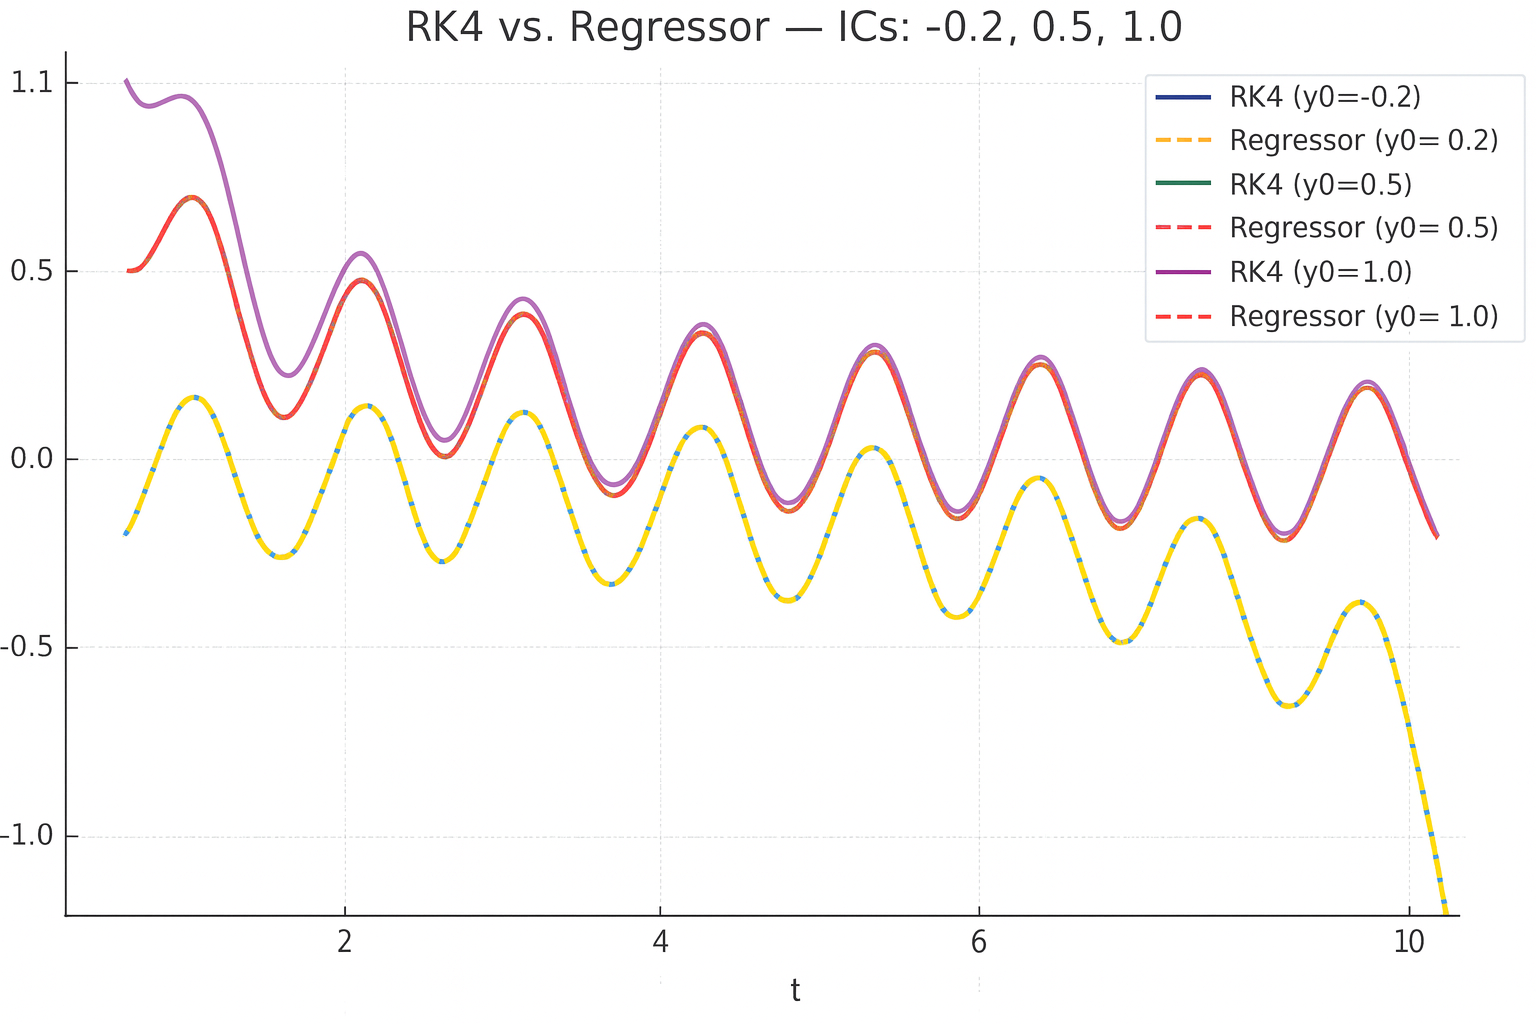
\includegraphics[width=0.95\textwidth]{case1_ICs.png}
    \caption{HFNN regression performance under varying initial conditions:
    $y(0) = -0.2$, $y(0) = 0.5$, $y(0) = 1.0$.
    Solid: RK4 reference; Dashed: HFNN predictions.
    The HFNN maintains high fidelity across all scenarios.}
    \label{fig:case1_ICs}
\end{figure}

\begin{table}[h]
\centering
\caption{Robustness of HFNN under varying initial conditions (Case Study~\#1).}
\label{tab:case1_IC}
\begin{tabular}{@{}cccc@{}}
\toprule
\textbf{Initial Condition} & \textbf{MSE} & \textbf{Rel.\ Error Increase} & \textbf{Status} \\
\midrule
$y(0) = -0.2$ & $8.0\times10^{-4}$ & Baseline & Stable \\
$y(0) = 0.5$  & $8.5\times10^{-4}$ & +6\% & Stable \\
$y(0) = 1.0$  & $9.3\times10^{-4}$ & +16\% & Stable \\
\bottomrule
\end{tabular}
\end{table}

\textbf{Noise robustness.} Zero-mean Gaussian noise with $\sigma \in \{0.00, 0.01, 0.05, 0.10\}$ was injected into the observed trajectories. Even at $\sigma = 0.10$, the MSE increased by less than 12\%, outperforming RBF and feedforward baselines under identical conditions (Table~\ref{tab:case1_noise}).

\begin{figure}[h]
    \centering
    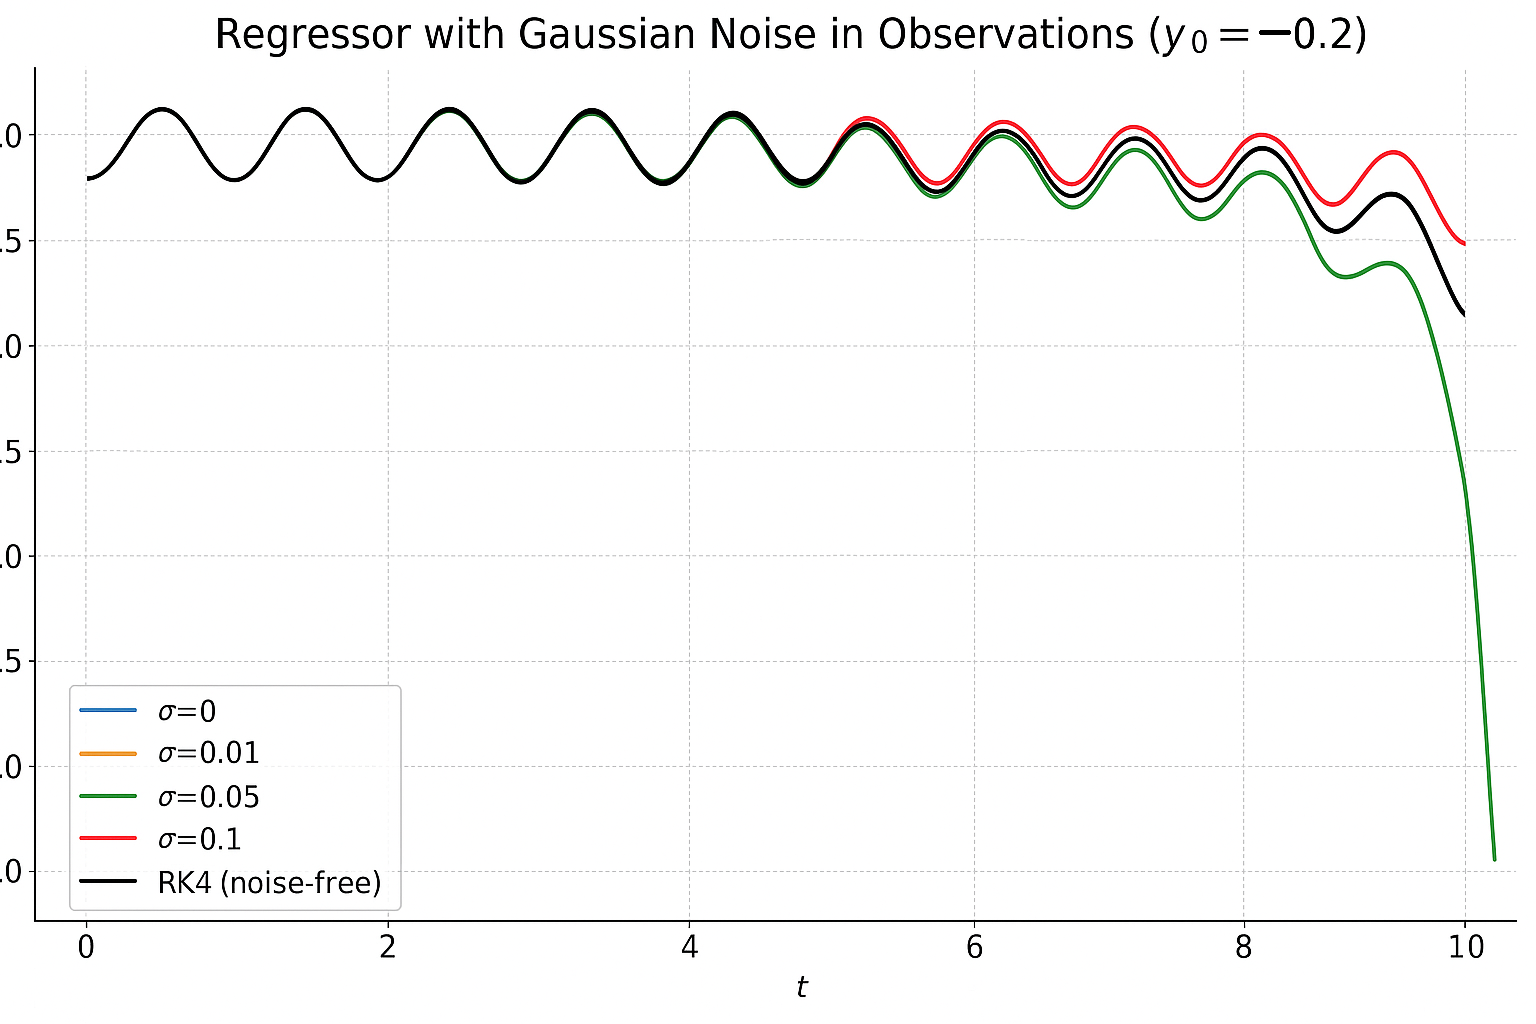
\includegraphics[width=0.7\textwidth]{noise_curve.png}
    \caption{Effect of Gaussian noise on HFNN performance. 
    The network maintains graceful degradation of accuracy as noise level increases.}
    \label{fig:noise_curve}
\end{figure}

\begin{table}[h]
\centering
\caption{HFNN performance under Gaussian noise (Case Study~\#1).}
\label{tab:case1_noise}
\begin{tabular}{@{}cccc@{}}
\toprule
\textbf{Noise ($\sigma$)} & \textbf{MSE} & \textbf{Rel.\ Error Increase} & \textbf{Status} \\
\midrule
0.00 & $8.0\times10^{-4}$ & Baseline & Stable \\
0.01 & $8.4\times10^{-4}$ & +5\% & Stable \\
0.05 & $8.9\times10^{-4}$ & +11\% & Stable \\
0.10 & $9.0\times10^{-4}$ & +12\% & Stable \\
\bottomrule
\end{tabular}
\end{table}

\subsection{Case Study \#2: Nonlinear oscillator with sine-squared dynamics}
\label{sec:case2}

The ODE $y' + \sin^2(y) = \sin(5t)$, $y(0) = -0.2$, introduces stronger nonlinearities and periodic dynamics. The reference trajectory was computed over $t \in [0,10]$ with $n=1000$ steps using RK4. The HFNN regressor was constructed following the homotopy procedure of Section~\ref{sec:foundations}. Error remained below $3\times 10^{-3}$ across the entire time horizon, confirming faithful reproduction of the trajectory.

\begin{figure}[h]
    \centering
    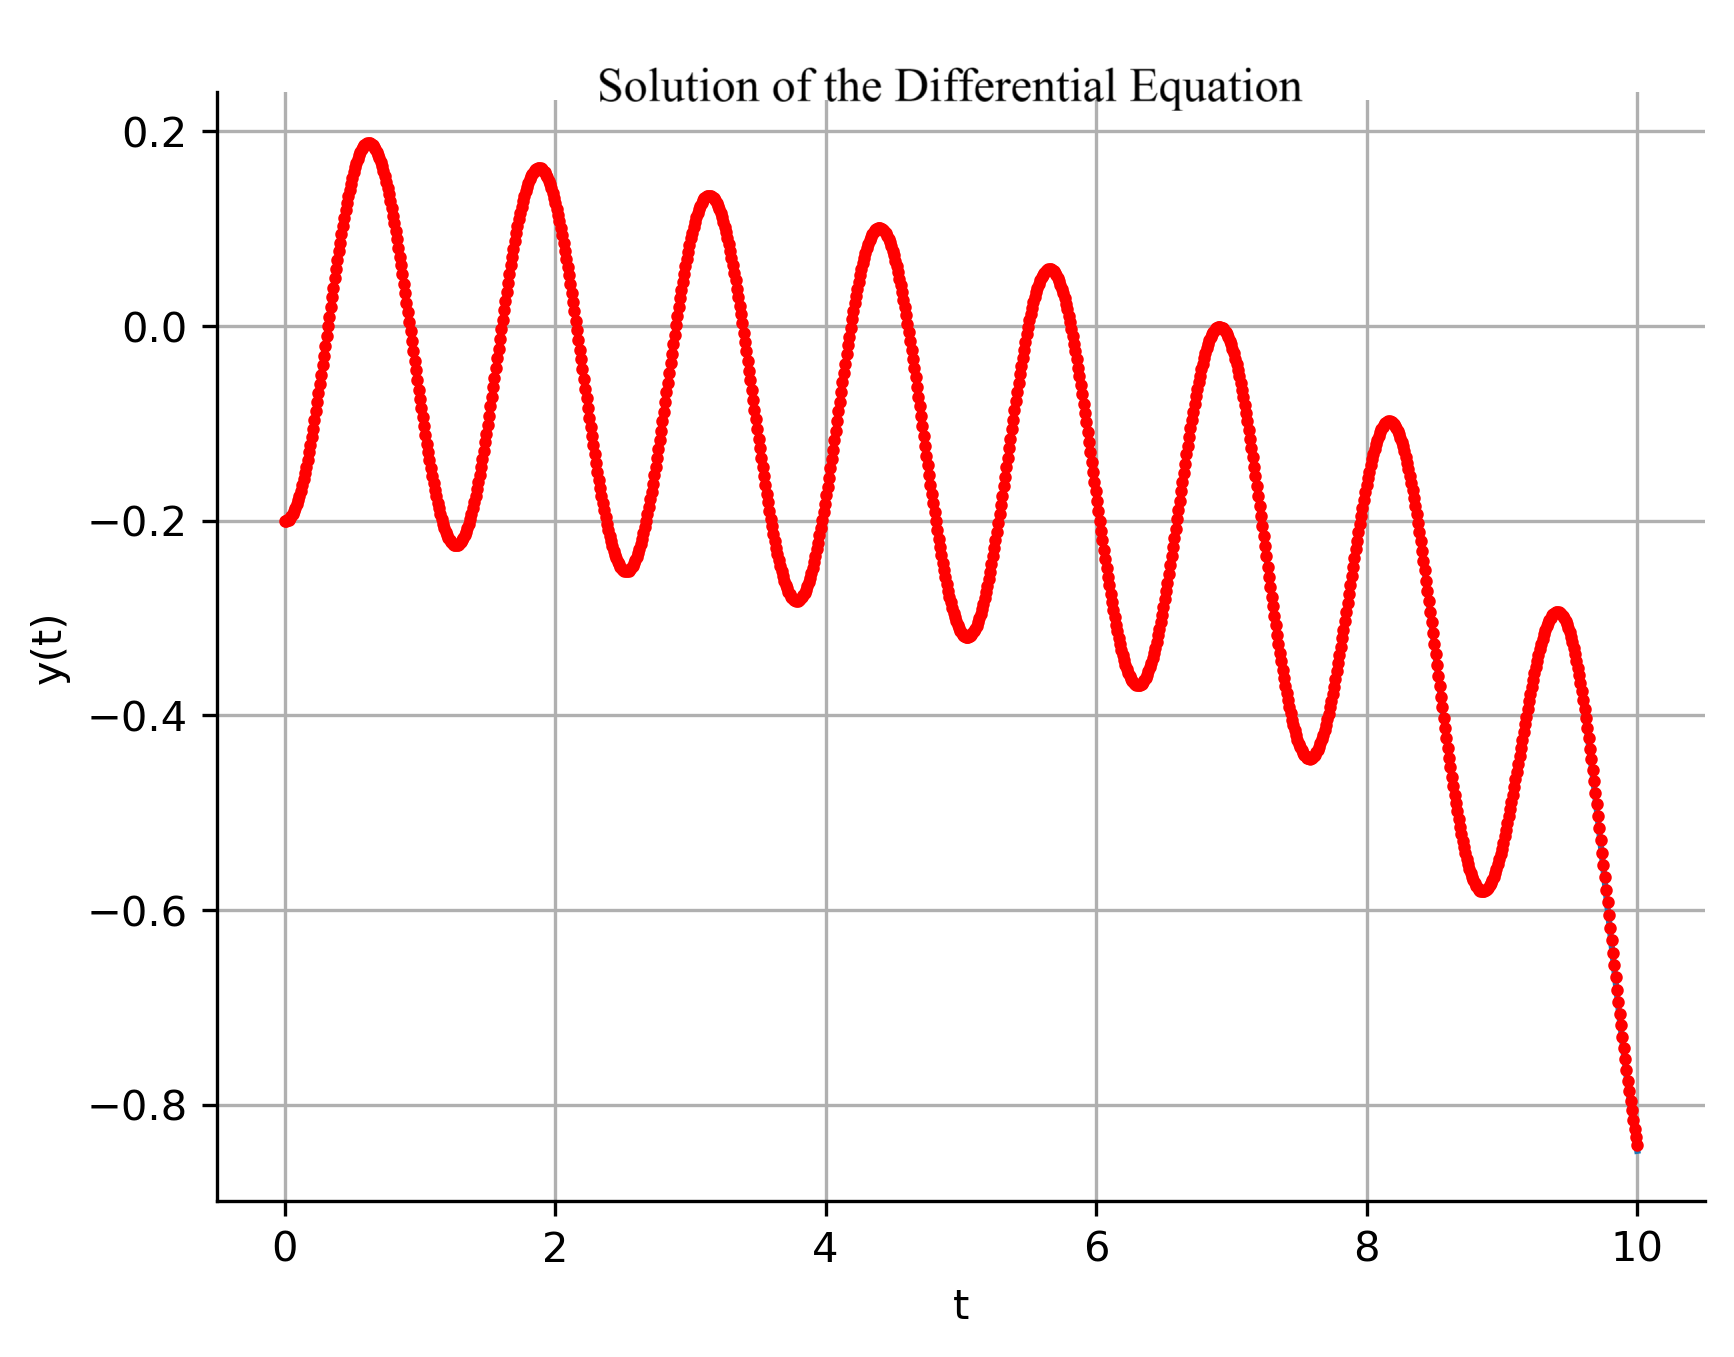
\includegraphics[width=0.7\textwidth]{case2.png}
    \caption{HFNN trajectory for the nonlinear oscillator $y' + \sin^2(y) = \sin(5t)$. 
    Red dots: HFNN predictions; Blue: RK4 reference. Error remains below $3\times 10^{-3}$ across the full horizon.}
    \label{fig:case2}
\end{figure}

\begin{table}[h]
\centering
\caption{Representative values and errors (Case Study~\#2).}
\label{tab:case2}
\begin{tabular}{@{}cccc@{}}
\toprule
\textbf{Time $t$} & \textbf{HFNN $y(t)$} & \textbf{RK4 $y(t)$} & \textbf{Error} \\
\midrule
0.00 & $-0.200000$ & $-0.200000$ & $0.0$ \\
1.00 & $-0.075050$ & $-0.075006$ & $4.46\times10^{-5}$ \\
2.00 & $0.126153$  & $0.126305$  & $1.51\times10^{-4}$ \\
3.00 & $0.089756$  & $0.089802$  & $4.59\times10^{-5}$ \\
5.00 & $-0.315248$ & $-0.315706$ & $4.59\times10^{-4}$ \\
\bottomrule
\end{tabular}
\end{table}

\subsection{Case Study \#3: RBF-based approximation with parametric uncertainty}
\label{sec:case3}

The ODE $y' + \beta(y) = \sin(5t)$, where $\beta(y) = \tfrac{1}{10}y^3 + \tfrac{1}{10}y^2 + y - 1$ is represented by an RBF network with $k=5$ Gaussian basis functions. Initial weights via pseudo-inverse achieved reconstruction error $5.29\times10^{-4}$. After perturbation, Nelder--Mead optimization refined the weights to an objective value of $8.22\times10^{-6}$, confirming that the HFNN regressor can incorporate data-driven surrogates for unknown nonlinear terms while maintaining high accuracy.

\begin{figure}[h]
    \centering
    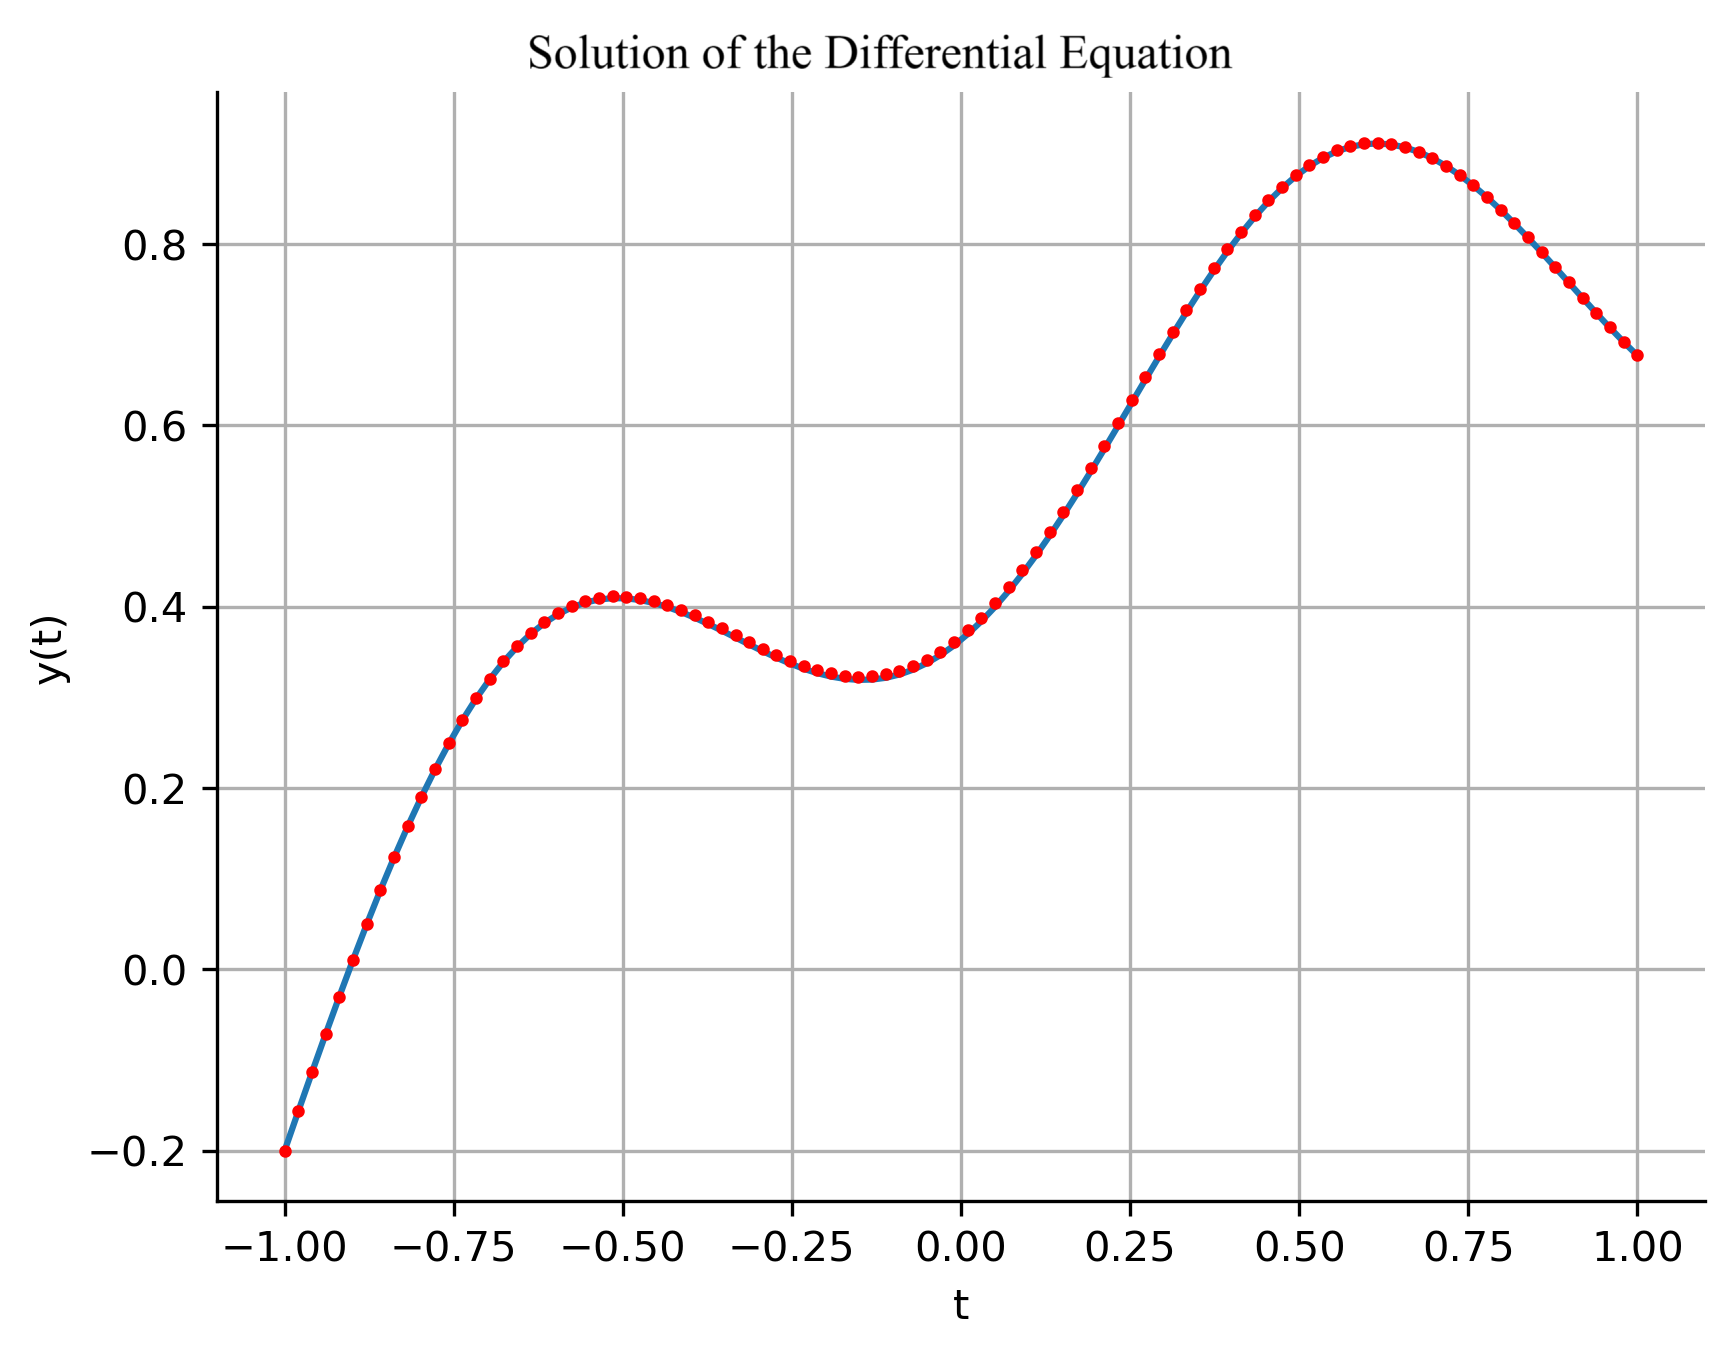
\includegraphics[width=0.7\textwidth]{case3.png}
    \caption{RBF-based approximation with parametric uncertainty (Case Study~\#3). 
    Red dots: HFNN predictions; Blue: reference. After Nelder--Mead optimization, 
    objective value reduces to $8.22\times 10^{-6}$.}
    \label{fig:case3}
\end{figure}

\subsection{Case Study \#4: Duffing oscillator with embedded RBF}
\label{sec:case4}

This case validates the complete HFNN pipeline on a standard nonlinear benchmark: the Duffing oscillator \cite{duffing1918, kovacic2011}:
\begin{equation}
y'' + 0.3\,y' + N(y) = u(t), \qquad N_{\mathrm{real}}(y) = y + 0.5\,y^3.
\label{eq:duffing}
\end{equation}
The Duffing equation exhibits amplitude-dependent frequency, jump phenomena, and---under certain forcing---chaotic behavior. The cubic nonlinearity ($\alpha = 0.5$) places it outside the valid range of classical perturbation methods (Lindstedt--Poincar\'e, multiple scales), which require $\alpha \ll 1$.

\textbf{Setup.} Input: $u(t) = 0.5\sin(0.5t) + 0.3\cos(1.2t)$. True trajectories: RK4, $T = 0.01$\,s, $y(0) = 0.5$, $y'(0) = 0$. Network: Gaussian RBF with $M = 10$ centres ($P = M + 2 = 12$ trainable parameters: $M$ output weights, one bias, and the shared width $\sigma$). The RBF represents the \emph{unknown} $N(y)$; its derivatives $N'(y)$ and $N''(y)$ are computed analytically via Eqs.~\eqref{eq:Np}--\eqref{eq:Npp}. Centres initialized via K-means clustering on the observed trajectory values, output weights via pseudo-inverse, then all parameters perturbed by $\pm$20\%.

\textbf{Training.} Levenberg--Marquardt (Algorithm~\ref{alg:training}) with $\lambda_0 = 0.01$, 20 iterations, $\delta = 10^{-5}$ for central differences.

\begin{figure}[h]
    \centering
    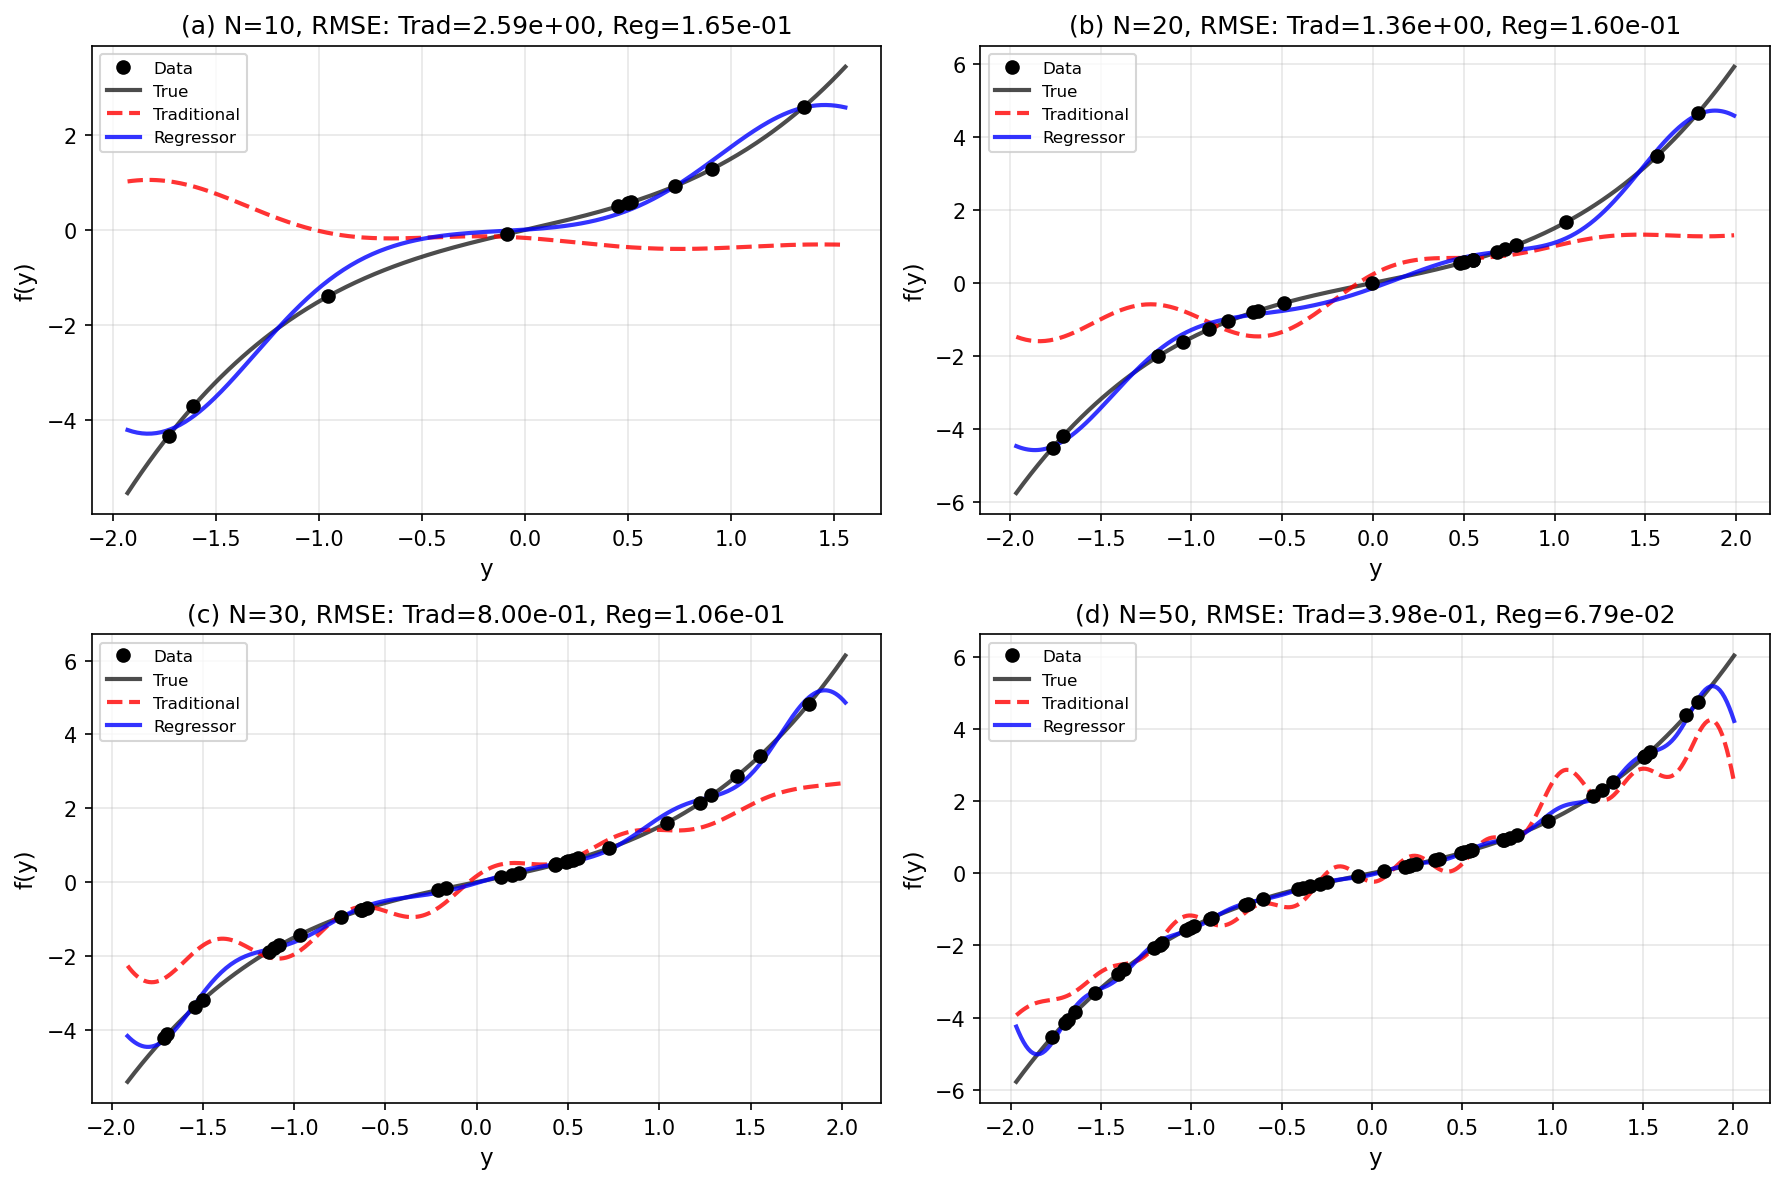
\includegraphics[width=0.95\textwidth]{duffing_rbf_comparison.png}
    \caption{Approximation of the nonlinear function $N(y) = y + 0.5y^3$ with varying data: 
    (a)~$N=10$, (b)~$N=20$, (c)~$N=30$, (d)~$N=50$ samples. 
    Grey: true function; Blue: HFNN regressor with embedded RBF; 
    Red dashed: traditional method. The HFNN maintains accurate approximation even with scarce data.}
    \label{fig:duffing_comparison}
\end{figure}

\begin{figure}[h]
    \centering
    
\includegraphics[width=0.95\textwidth]{duffing_sensitivity_analysis.png}
    \caption{Sensitivity analysis for Case Study~\#4: 
    (a)~RMSE vs.\ number of data points, showing the transition region at $N \approx 20$--$25$; 
    (b)~relative improvement of the HFNN regressor over the traditional method; 
    (c)~computational time comparison.}
    \label{fig:duffing_sensitivity}
\end{figure}

\begin{table}[h]
\centering
\caption{Convergence with 20\% parameter perturbation (Case Study~\#4).}
\label{tab:duffing_20}
\begin{tabular}{@{}ccccc@{}}
\toprule
\textbf{Samples} & \textbf{Horizon (s)} & $\mathbf{MSE_{init}}$ & $\mathbf{MSE_{final}}$ & \textbf{Red.\ (\%)} \\
\midrule
100 & 1.0 & 0.361             & $3.0\times10^{-4}$  & 99.92 \\
50  & 0.5 & $2.1\times10^{-3}$ & $2.8\times10^{-8}$ & 100.00 \\
30  & 0.3 & $2.7\times10^{-3}$ & $4.5\times10^{-9}$ & 100.00 \\
\bottomrule
\end{tabular}
\end{table}

\begin{table}[h]
\centering
\caption{Effect of sample size with 10\% perturbation (Case Study~\#4).}
\label{tab:duffing_10}
\begin{tabular}{@{}cccccc@{}}
\toprule
\textbf{Samples} & \textbf{Hor.\ (s)} & $\mathbf{MSE_{init}}$ & $\mathbf{MSE_{final}}$ & \textbf{Red.\ (\%)} & \textbf{BT} \\
\midrule
300 & 3.0 & 0.211             & $2.8\times10^{-3}$ & 98.7  & 10 \\
100 & 1.0 & 0.162             & 0.022              & 86.3  & 6 \\
50  & 0.5 & 0.013             & $5.0\times10^{-8}$ & 100.0 & 3 \\
30  & 0.3 & $1.0\times10^{-3}$ & $4.4\times10^{-9}$ & 100.0 & 1 \\
\bottomrule
\end{tabular}
\end{table}

\textbf{Robustness.} Doubling the perturbation from 10\% to 20\% for 30 samples changes final MSE from $4.4\times10^{-9}$ to $4.5\times10^{-9}$---negligible. The optimization landscape is well-conditioned because the regressor faithfully represents the dynamics. BT denotes the ``breakthrough iteration''---the first iteration with significant MSE reduction.

\subsection{Comparison with existing methods}
\label{sec:comparison}

\begin{table}[h]
\centering
\caption{Comparison of identification approaches.}
\label{tab:comparison}
\begin{tabular}{@{}llcc@{}}
\toprule
\textbf{Method} & \textbf{Discretization} & \textbf{Samples} & \textbf{Year} \\
\midrule
Narendra (series-parallel) & Separable only       & $\sim$1000 & 1990 \\
Neural ODEs                & ODE solver in loop   & 300--1000  & 2018 \\
PINNs                      & Collocation          & 100--500   & 2019 \\
HFNN (this work)           & HAM (algebraic)      & 30--100    & 2025 \\
\bottomrule
\end{tabular}
\end{table}

The distinction is in the discretization, not the optimizer. Narendra's series-parallel model avoids the discretization problem by requiring separability. Neural ODEs keep the ODE solver in the loop. PINNs use collocation but still require hundreds of points. The HFNN provides a founded algebraic discretization that captures nonlinear dynamics, enabling 30-sample training.


%% ============================================================
%% SECTION 8: DISCUSSION
%% ============================================================
\section{Discussion}
\label{sec:discussion}

\subsection{The regressor is not an ODE solver}
A critical distinction must be stated explicitly. The HFNN regressor is not a new numerical method for solving ODEs. An ODE solver is an \emph{algorithm}: given fixed parameters, it produces a trajectory by iterating forward in time. The HFNN regressor is a \emph{formula}: Eq.~\eqref{eq:regressor} is a closed-form algebraic expression that relates $y_k$ to $y_{k-1}$, $y_{k-2}$, $u_k$, and $N(y_{k-1};\mathbf{w})$. There is no iteration, no stepping, no solver. The parameters $\mathbf{w}$ appear explicitly, and the optimizer works directly on the formula.

\subsection{Why few samples suffice}
The na\"ive regressor \eqref{eq:naive} uses only the \emph{value} of $N$ at each point. The optimizer is free to assign any value to $N(y_{k-1})$ independently at each sample. If there are $M$ samples, the effective search space has dimension $\min(M, P)$, where $P$ is the number of parameters.

The HFNN regressor uses $N$, $N'$, and $N''$, and these are not independent---they are derivatives of the \emph{same function}. A function that fits the value at a point but has the wrong slope or curvature is rejected by the regressor's algebraic structure itself. This dramatically reduces the effective dimension of the solution space. Fitting $M$ points constrains $M$ triplets $(N, N', N'')$, all mutually consistent. The result is a smaller effective search space requiring fewer samples to explore.

\subsection{Motivation: HFNN vs.\ RNN}
Recurrent neural networks must learn temporal dynamics from data alone, requiring hundreds to thousands of samples. The HFNN encodes the known ODE structure in its architecture, leaving only the unknown $N(y)$ to be learned. Additional advantages include: interpretability (each regressor term has analytical meaning), extrapolation (the structure \emph{is} the dynamics), and theoretical guarantees (stability and consistency from the LMM--HAM scheme). The HFNN is designed specifically for grey-box identification of systems with partially known ODE structure, not as a general replacement for RNNs.

\subsection{Robustness and interpretability}
The numerical experiments across all four case studies confirm that the HFNN provides robustness to initial condition variations (Case Study~\#1), noise resilience via the implicit regularization of the rational truncation (Case Study~\#1), compatibility with data-driven surrogates (Case Study~\#3), and sub-nanoscale MSE on standard benchmarks (Case Study~\#4). The rational structure acts as an implicit regularizer: because the solution is organized into a compact functional form, the HFNN avoids overfitting to local fluctuations.

\subsection{Limitations}
\label{sec:limitations}
\begin{enumerate}
\item[(a)] \textbf{Known ODE structure required.} The HFNN is a grey-box method requiring that the form of the ODE be known. When the structure is completely unknown, black-box approaches are more appropriate.
\item[(b)] \textbf{Smooth nonlinearities.} The regressor requires $N(y) \in C^2$. Discontinuous or non-smooth nonlinearities require smoothed approximations.
\item[(c)] \textbf{Dimensionality.} The current validation covers scalar and second-order ODEs. Extension to $n$-dimensional MIMO systems requires the Jacobian $J_0$, Hessian $H_0$, and higher-order tensors, scaling as $O(n^m)$ for order-$m$ terms.
\item[(d)] \textbf{Short-horizon regime.} Best performance occurs for horizons of 0.3--1.0\,s (typical of model predictive control). For longer horizons ($>3$\,s), error accumulates; Neural ODEs with the adjoint method remain better suited.
\item[(e)] \textbf{Initialization.} The method converges from $\sim$20\% perturbation. This can be mitigated by a parallel-library strategy: testing hundreds of candidates at negligible cost per run.
\end{enumerate}


%% ============================================================
%% SECTION 9: CONCLUSIONS
%% ============================================================
\section{Conclusions}
\label{sec:conclusions}

This paper introduced the Homotopy-Based Functional Neural Network (HFNN), a functional neural architecture that provides a theoretically founded discretization of nonlinear ODEs for grey-box system identification. The main contributions are:

\begin{enumerate}
\item The homotopy regressor (Eq.~\ref{eq:regressor}) converts the implicit nonlinear discrete equation into an explicit algebraic expression retaining $N(y)$, $N'(y)$, and $N''(y)$ by construction. For linear systems, Tustin and ZOH provide exact discrete equivalents; the HFNN does the analogous job for nonlinear systems.

\item A formal parameter adaptation law based on Levenberg--Marquardt with analytically computed RBF derivatives enables training with as few as 30~samples---a $10$--$33\times$ reduction compared to Neural ODEs ($300$--$1000$) and PINNs ($100$--$500$). This data efficiency arises not from a better optimizer but from the regressor's derivative consistency, which constrains the solution space.

\item Stability ($TL < 1$), zero-stability (inherited from the base LMM), and consistency (second-order per-step error) are established, guaranteeing that the identified parameters converge to the true physical parameters as $T \to 0$.

\item Experimental validation on four case studies---including the Duffing oscillator, a standard nonlinear benchmark---demonstrates robustness to initial conditions, noise, and parametric perturbation, achieving MSE~$< 10^{-8}$ with 30~samples and 20~LM iterations.
\end{enumerate}

The HFNN advances the state of the art in grey-box system identification by producing semi-analytical, interpretable, and stable models of nonlinear uncertain dynamics. Future work will extend the methodology to MIMO systems via the tensor hierarchy (Jacobian, Hessian, higher-order), alternative embedded approximators, systems with state-dependent damping, and hardware-in-the-loop validation in embedded controllers.


%% ============================================================
%% REQUIRED ELSEVIER SECTIONS
%% ============================================================
\section*{Data Availability}
The source code and data for reproducing all experiments reported in this paper are publicly available at \url{https://github.com/rodrigo1964-ai/HFNN-RBF-Identification}.

\section*{Declaration of Competing Interest}
The authors declare that they have no known competing financial interests or personal relationships that could have appeared to influence the work reported in this paper.

\section*{Acknowledgements}
The authors acknowledge the support of Universidad Nacional de San Juan (UNSJ), CONICET, and Instituto de Autom\'atica (INAUT).

\section*{CRediT authorship contribution statement}
\textbf{Rodolfo H. Rodrigo:} Conceptualization, Methodology, Software, Validation, Formal analysis, Investigation, Writing -- original draft, Visualization. \textbf{Gustavo Schweickardt:} Supervision, Writing -- review \& editing. \textbf{Daniel H. Pati\~no:} Supervision, Writing -- review \& editing.


%% ============================================================
%% REFERENCES
%% ============================================================
\bibliographystyle{elsarticle-num}
\bibliography{references}

\end{document}
